\chapter{Single Particle}
\label{ch:sp}

\section{System and Hamiltonian}
\label{sec:sp:sysh}

We begin by considering a dielectric particle with mass $m$,
    radius $R$,
    and polarizability $\alpha$.
This nanoparticle is trapped by optical tweezers inside an optical cavity of length $L$.
We choose the $x$-axis to align with the polarization of the laser,
    the $+z$-axis to be in the propagation direction of the tweezers
    and the $y$-axis to align with the cavity axis.
The origin is chosen to be at the intensity maximum of the tweezers. 
In this thesis we assume that $R \ll \lambda$ 
    and we can treat the particle as a point mass compared to the wavelength.

The tweezers have a frequency $\omega_0$, a power of $P_t$, and a waist $W_t$ at the focus.
A sketch of the setup can be seen in Figure \ref{fig:sp:setup}.

\begin{figure}
    \centering
    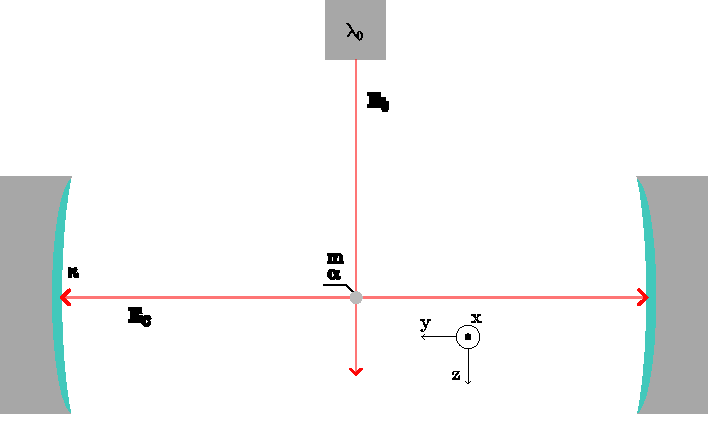
\includegraphics[width=0.8\linewidth]{chapters/10_single_cavity/sketch.pdf}
    \caption{
        Sketch of the setup\\
        From above we have a Laser with the wavelength $\lambda_0$.
        %The electric field of the Laser is described by $\vec E_t$.
        %\\
        On the sides we have two optical mirrors that form a Cavity.
        %Their damping effects are described by $\kappa$.
        %The field inside the cavity is described by $\vec E_c$.
        %\\
        The gray point describes the dielectric particle, 
            %with polarizability $\alpha$ and mass $m$
    }
    \label{fig:sp:setup}
\end{figure}

With this, our Hamiltonian for a particle at the position $\vec r$ at the time $t$ is
\begin{equation}
\label{eq:sp:Hprim}
    H = \frac{\norm{\vec{p}}^2}{2m} - \frac1 2 \vec{ d } \cdot \vec E_{tot}(t, \vec r) + H_c 
    = \frac{\vec{p}^2}{2m} - \frac\alpha2 \norm{\vec E_{tot}(t, \vec r)}^2 + H_c.
\end{equation}
This is because the dipole moment $\vec d$ can be written as
\begin{equation}
    \vec d = \alpha \vec E_{tot}.
\end{equation}
Here $\vec p$ is the momentum of the particle, 
    $\vec E_{tot}$ is the total electric field
    and $H_c$ is the cavity Hamiltonian.
This also induces the non-linear self-interaction of the particle with the field.

\section{Cavity Hamiltonian}
\label{ssec:sp:Hc}

In Equation \eqref{eq:sp:Hprim} $H_c$ represents the energy stored in the cavity 
    and can be written as
\begin{equation}
    H_c = \frac 1 2 \iiint_{\R^3} d^3 r \left[ 
        \frac{\norm{\vec D}^2}{\epsilon_0} 
        + \frac{\norm{\curl \vec A}^2}{\mu_0} 
    \right],
\end{equation}
with $\vec D$ being the electric displacement field, 
    $\vec A$ being the vector potential,
    $\epsilon_0$ being the vacuum permittivity and $\mu_0$ the vacuum permeability.

Following Reference \cite{Maurer_2023} the fields in $H_c$ can be decomposed as
\begin{align}
\label{eq:sp:decomp:1}
    \vec A &= \sum_\beta \vec A_\beta(\vec r) A_\beta(t)
\end{align}
    and 
\begin{align}
    \vec D &=  \sum_\beta \vec A_\beta(\vec r) \epsilon(\vec r)D_\beta(t),
\label{eq:sp:decomp:2}
\end{align} 
here $\beta$ labels the specific mode of the EM field in the presence of the cavity,
    $\vec A_\beta(\vec r)$ being the stationary waves of the vector field 
    and $A_\beta(t) = \exp(i\omega_\beta t)$ being the corresponding time evolution.
The displacement field $\vec D_\beta$ is equal to $\epsilon(\vec r) \vec A_\beta$ following maxwells equations,
    with $\epsilon(\vec r)$ permittivity of the medium at the position $\vec r$.
The steady state solutions remain, 
    while the time evolution may be different, so the time evolution is given by $D_\beta(t)$.

The spacial field $\vec A_\beta(\vec r)$ also satisfies
\begin{equation}
    (\vec A _\beta, \vec A_\gamma)_{\epsilon(\vec r)} 
        = \iiint_{\R^3} d^3 r~
            \epsilon(\vec r) \vec A_\beta(\vec r) \cdot \vec A_\gamma(\vec r)
        = \delta_{\beta\gamma}
\end{equation}
    and the time dependent field satisfies
\begin{equation}
    \partial_tA_\beta(t) = i\omega_\beta A_\beta.
\end{equation}
The mode functions are determined such that each partial $\vec A_\beta(\vec r) A_\beta(t)$ is a solution of the Helmholtz-Equation
\begin{align}
    \curl \curl \vec A_\beta(\vec r) A_\beta(t) &=
       -\frac1 {c^2} \partial_t^2 \vec A_\beta(\vec r) A_\beta(t) \\
        &=~ \frac{\omega_\beta^2}{c^2} \vec A_\beta(\vec r) A_\beta(t).
\end{align}

To simplify the Hamiltonian,
    we use the algebraic property
\begin{equation}
(\curl \vec f)\cdot (\curl \vec g) = 
    \vec f\cdot(\curl\curl \vec g)
    - \div (\vec f \times (\curl \vec g)),
\end{equation}
which gives the form
\begin{equation}
    H_c = \frac{1}{2} \sum_\beta \left[ 
        \frac{D_\beta^2(t)}{\epsilon_0} 
        + \epsilon_0 \omega_\beta A_\beta^2(t)
    \right].
\end{equation}

As shown by Reference \cite{Gonzalez_Ballestero_2019},
    the cavity is almost in resonance with the field,
    so we can approximate the system by limiting it to a single  mode,
    this allows us to write the Hamiltonian as
\begin{equation}
    H_c = \frac{D_c^2(t)}{2\epsilon_0} 
        + \frac{1}{2}\epsilon_0 \omega_c A_c^2(t).
\end{equation}

We transform to the new coordinates $(a, a^*)$, 
    to simplify our system.
The new coordinates are defined by
%\footnote{
%    This is very similar to how the ladder operators are defined in Quantum mechanics. 
%    As such, they provide similar behavior with the Poisson brackets.
%}
\begin{align}
    A_c(t) 
        &= \sqrt{\frac{\hbar}{2\epsilon_0 \omega_c}}\Re\left\{a_c(t)\right\} 
         =  \sqrt{\frac{\hbar}{2\epsilon_0 \omega_c}} \left(a_c(t) + a_c^*(t)\right) 
\end{align}
and 
\begin{align}
D_c(t) 
        &= \sqrt{\frac{\hbar \epsilon_0 \omega_c}{2}} \Im\left\{a_c(t)\right\}
         = -\i\sqrt{\frac{\hbar \epsilon_0 \omega_c}{2}} (a_c(t) - a_c^*(t)).
\end{align}
Substitution gives the cavity Hamiltonian 
\begin{equation}
    H_c = \hbar \omega_c a_c^*(t)a_c(t).
\end{equation}

The new coordinates do not satisfy the canonical relations. 
However, they only differ by a constant factor of $\i \hbar$, 
    we may rescale the Poisson brackets to accommodate this.
Thus, the new equations of motion are
\begin{align}
\label{eq:sp:eom:adot}
    \dot a(t) &= \{a_c^*, H\} = -\frac{\i}{\hbar} \frac{\partial H}{\partial a_c^*}
\end{align}
    and
\begin{align}
    \dot a^*(t) &= \{a_c, H\} = +\frac{\i}{\hbar} \frac{\partial H}{\partial a_c}.
\end{align}

From the equations of motion, we can observe that this is a non-canonical transform, 
    and does change the symplectic structure.
The equations of motion can be used to write a new symplectic structure, 
    which is defined by
\begin{equation}
    \{\eta_i, \eta_j\} = J_{ij}
\end{equation}
which gives us
\begin{equation}
    \mat{J} = \frac{1}{\i\hbar} \begin{pmatrix}
        0 & 1 \\
        -1 & 0
    \end{pmatrix}
\end{equation}
for the subspace $[a_c, a_c^*]$.
This allows the equations of motion to be written as
\begin{align}
    \begin{pmatrix}
        a_c \\a_c^*
    \end{pmatrix} &= \mat{J} \cdot \grad_{[a_c, a^*_c]}H
\end{align}
for the subspace.

\section{Model of the fields}
\label{sec:sp:model}

The modeling of this system was done in Reference \cite{Gonzalez_Ballestero_2019} in a QFT framework,
    in this thesis,
    this is adapted into a classical view.
\par

The total electric field can be written as
\begin{equation}
    \vec E_{tot}(\vec r) = \vec E_t(\vec r, t) + \vec E_c(\vec r).
\end{equation}

\subsection{Tweezers field}
\label{ssec:sp:model:tweezer}

For optical tweezers, we define them to have a Gaussian structure \cite{PhysRevE.49.5778},
    and thus we can write
\begin{equation}
\label{eq:sp:vEt}
    \vec E_{tot}(\vec r, t) = \vec e_xE_t(\vec r) \exp(-\i\omega_0 t) +c.c.
\end{equation}
with the additional scalar function
\begin{equation}
\label{eq:sp:Et}
    E_t(\vec r) = \frac{E_0}{2} \exp(\i(k_0z + \phi_t(\vec r))) \frac{W_t}{W(z)}
        \exp\left(-\left[ \frac{y}{A_y W(z)} \right]^2\right)
        \exp\left(-\left[ \frac{x}{A_x W(z)} \right]^2 \right)
\end{equation}
where $W_t$ is the waist of the tweezers,
    $W(z) = W_t \sqrt{1+(z/z_R)^2}$, 
    and the Gouy phase is defined as
\begin{equation}
    \phi_t(\vec r) = - \arctan{(z/z_R)} + \frac{k_0z}{2} \frac{x^2+y^2}{z^2+z_r^2}
\end{equation}
with $z_R = \pi W_t^2/\lambda_0$ being the Rayleigh range.
In general, the beam may be asymmetric in the $x$ and $y$ directions,
    to include this in the model the parameters of $A_{x,y}$ are introduced.

The field amplitude is written in terms of the power as 
\begin{equation}
\label{eq:sp:Et0}
    E_0 = \sqrt{\frac{4 P_t}{\pi \epsilon_0 c W_t^2 A_x A_y}}.
\end{equation} 

\subsection{Cavity field}
\label{ssec:sp:model:cavity}

The structure of the Cavity field is already defined by the decomposition we used.
From the definition of the displacement field
\begin{equation}
\label{eq:sp:vEc:prim}
    \vec E_c(\vec r, t) 
        = \frac{\vec D_c(\vec r, t)}{\epsilon_0\epsilon(\vec r)} 
        = \frac{\vec A_c(\vec r) D_c(t)}{\epsilon_0}
\end{equation}
    and our definition of $D_c(t) \propto \Re{a_c}$,
    there exists a function $E_c(\vec r)$
    that allows us to express the total cavity field as
\begin{equation}
\label{eq:sp:vEc}
    \vec E_c(\vec r, t) = \vec e_x E_c(\vec r) a_c + c.c. .
\end{equation}

Given the solutions of $\vec A_\alpha(\vec r)$ this gives us
\begin{equation}
    \label{eq:sp:Ec}
    E_c(\vec r) = E_{0,c} \exp(-(x^2+z^2)/W_c^2) \zeta \cos(k_c y) \in \R,
\end{equation}
and the zero-point field strength of
\begin{equation}
    \label{eq:sp:Ec0}
    E_{0, c} = \sqrt{\frac{\hbar \omega_c}{2\epsilon_0 V_c}}.
\end{equation}
Similar to the tweezers $W_c$ represents the waist of the Gaussian.
The mode Volume is given by $V_c = \pi W_c^2 L_c /4$ with the cavity length $L_c$,
    and we also denote $k_c = \omega/c$ as the cavity wave number.
For a solution $E_t$ its negative is also a solution
    to model this we include the parameter of $\zeta = \pm 1$.


\subsection{Time Averaging}
\label{ssec:sp:model:timeavg}

The full expression for $\norm{\vec E_{tot}}$ is
\begin{equation}
    \norm{\vec E_{tot}} = \norm{\vec \varepsilon_t}^2 + \norm{\vec E_c}^2 + 2|\vec \varepsilon_t \cdot \vec E_c|
\end{equation}
with
\begin{align}
    \norm{\vec \varepsilon_t}^2 &= E_t^2 \exp(-2\i\omega_0 t) 
        + E_t^{*2} \exp(2\i\omega_0 t) + 2|E_t|^2, \\
    \norm{\vec E_c}^2 &= E_c^2 a_c^2 + E_c^2 a^{*2}_c + 2E_c^2 |a_c|^2 = E_c^2 \alpha_c \alpha_c^* + E_c^2 \left(\alpha_c^2\exp(-2\i\omega_0t) + c.c. \right), 
\end{align}
and  
\begin{align}
|\vec \varepsilon_t \cdot \vec E_c| &= E_c(E_t \exp(-\i\omega_0 t) + c.c.) (\alpha_c \exp(-\i\omega_0 t)+c.c.) .
\end{align}
Here we define
\begin{equation}
    a_c := \alpha_c \exp(-\i \omega_0t)
\end{equation}

To eliminate very fast-changing terms
    we take the time average of the time $T = \pi/\omega_0$.
The fast changing terms vanish as we integrate over a period
    and for the slower changing terms the time averaging acts like a derivative and cancels the integral.
This yields
\begin{equation}
    \norm{\vec E_{tot}(\vec r)}^2 = 2\left(
        |E_t(\vec r)|^2  
        +  E_c^2(\vec r) a_c^* a_c
        +  \left[a_c E_cE_t^* \exp(i\omega_0 t) + c.c.\right]\right).
\end{equation}

\section{Equations of Motion}
\label{sec:sp:hameqs}

Using the above modeling and approximations
    the Hamiltonian can be written as
\begin{equation}
    H = \frac{\norm{\vec p}^2}{2m} 
        + \hbar \omega_c a_c^* a_c
        - \alpha \left[ \left|E_t(\vec r)\right|^2  +E_c^2(\vec r) a_c^* a_c
            + \left[a_c E_cE_t^* \exp(\i\omega_0 t) + c.c. \right]\right].
\end{equation}

Applying Equation \eqref{eq:sp:eom:adot} leads to
\begin{equation}
\label{eq:sp:dotat}
    \dot a_c(t) = -\i \left(\omega_c - \frac{\alpha}{\hbar} E_c^2(\vec r) \right)a_c + \frac{\i\alpha}{\hbar} E_t(\vec r)E_c(\vec r) \exp(-\i\omega_0 t).
\end{equation}

We use the canonical transform
\begin{equation}
    a_c(t) = \alpha_c(t)\exp(-\i\omega_0 t)
\end{equation}
to transform the Hamiltonian to be time independent.
Applying the transform gives
\begin{align}
\label{eq:sp:dotalpht}
    \dot \alpha_c(t) 
        &= -\i \underset{:=\delta_c}{\underbrace{\left(\omega_c -\omega_0 - \frac{\alpha}{\hbar} E_c^2(\vec r) \right) }}\alpha_c(t)
            + \frac{\i\alpha}{\hbar} E_t(\vec r)E_c(\vec r),
\end{align}
and with this transform the Hamiltonian can be expressed as
\begin{equation}
     H = \frac{\norm{\vec p}^2}{2m} 
        + \hbar \Delta \alpha_c^* \alpha_c
        - \alpha \left[ \left|E_t(\vec r)\right|^2  +E_c^2(\vec r) \alpha_c^* \alpha_c+ \left[
            \alpha_c E_cE_t^* + c.c. 
        \right]\right].
\end{equation}

This expression uses the detuning $\Delta$ defined as
\begin{equation}
\label{eq:sp:def:detuning}
    \Delta := \omega_c - \omega_0.
\end{equation}

Our goal is to determine the equilibrium values for all the classical amplitudes, $\vec r$ and $\alpha_c$.
At equilibrium the time derivative of these generalized coordinates needs to be set to $0$.
Applying this to the cavity field yields
\begin{equation}
    \alpha_c^{eq} = \frac{\alpha}{\hbar} 
        \frac{E_t(\vec r^{eq}) E_c(\vec r^{eq})}{\delta_c - i \frac{\kappa}{2}}.
\end{equation}
The extra term of $-i\kappa/2$ is included to model the loss of light, 
    due to imperfect mirrors,
     Reference \cite{Gonzalez_Ballestero_2019} shows that this gives a good description of damping.
The additional term is also needed to avoid divergence at $\Delta = 0$.

Applying the equilibrium condition to the particle position gives
\begin{equation}
    \ddot{\vec r} \propto \dot{\vec p} = -\grad_{\vec r}{H}
        = +\alpha \grad_{\vec r} |E_t(\vec r) + \alpha_c(t) E_c(\vec r)|^2 \overset{!}{=} \vec 0
\end{equation}
or equivalently
\begin{equation} 
        \grad
            |E_t(\vec r) + \alpha_c^{eq}(\vec r^{eq}) E_c(\vec r)|^2 |_{\vec r = \vec r^{eq}} 
            \overset{!}{=} \vec 0.
\end{equation}


\section{Finding the Extremes}
\label{sec:sp:extrem}

The identity $\grad |h|^2 = 2 \Re\{ h^* \grad h \}$
    can be utilized to rewrite the expression as
\begin{equation}
\label{eq:sp:extremes:init}
    \Re\{ (E_t^*(\vec r) + \alpha_c^{eq*} E_c(\vec r))
        (\grad E_t(\vec r) + \alpha_c^{eq} \grad E_c(\vec r))  \} \overset{!}{=}0.
\end{equation}

We can simplify the expression further, 
    by using the logarithmic derivatives
\begin{align}
    \vec f(\vec r) &= \grad \ln E_t(\vec r) \\
    \text{and }\vec g(\vec r) &= \grad \ln E_c(\vec r).
\end{align}

With those definitions, the Equation \eqref{eq:sp:extremes:init} can be rewritten as
\begin{align}
    &\Re\{ \left(E_t^*(\vec r^{eq}) + \alpha_c^{eq*} E_c(\vec r^{eq})\right)
        (\vec f(\vec r^{eq})E_t(\vec r^{eq}) + \alpha_c^{eq} \vec g(\vec r) E_c(\vec r))  \} \\
    &= |E_t|^2 \Re\left\{ \left(1 + 
            \frac{\alpha}{\hbar} \frac{ E_c^2}{\delta_c + i \frac{\kappa}{2}} \right)
        \left(\vec f +  
            \frac{\alpha}{\hbar} \frac{E_c^2}{\delta_c - i \frac{\kappa}{2}}
            \vec g \right)  \right\}(\vec r^{eq})  \\
    &\overset{!}{=}0.
\end{align}

From the model of the tweezers in  Section \ref{sec:sp:model} it is obvious that $|E_t|>0$ for all positions $\norm{\vec r} < \infty$,
    as such, it can be removed without missing any roots.

Thus, the expression can be written as
\begin{equation}
        \Re\left\{ \left(1 + 
            \gamma \left(\delta_c - \i \frac{\kappa}{2} \right) \right)
        \left(\vec f +  
            \gamma \left( \delta_c + \i\frac{\kappa}{2} \right)
            \vec g \right)  \right\} 
    \overset{!}{=}0.
\end{equation}
with 
\begin{equation}
    \gamma := \frac{\alpha}{\hbar} \frac{ E_c^2(\vec r^{eq})}{\delta_c^2 +\frac{\kappa^2}{4}} \in \R.
\end{equation}

Using the property that $\Re \{z_1z_2\} = \Re z_1 \Re z_2 - \Im z_1\Im z_2$ this becomes
\begin{equation}
    \left( 1+\gamma \delta_c\right)
        \left( \Re \vec f + \vec g \gamma \delta_c \right) 
    + \gamma \frac{\kappa}{2} 
        \left( \Im \vec f + \vec g \gamma \frac{\kappa}{2}\right) \overset{!}{=}0.
        \label{eq:sp:equiv:vec}
\end{equation}
This expression cannot be simplified further in vector form.
Thus, we continue to find solutions for the individual components.

\subsection{\texorpdfstring{$x$}{x}-Component}
\label{ssec:sp:extrem:x}

Based on the fields in equations \eqref{eq:sp:Et} and \eqref{eq:sp:Ec}
    the $x$-component of the logarithmic gradients are
\begin{align}
    f_x &= x \left[ \i\frac{k_0z}{z^2+z_R^2} - \frac{2}{A_x^2 W^2(z)}\right] 
\end{align}
and 
\begin{align}
    g_x &= -\frac{2x}{W_c^2}.
\end{align}

Substitution into Equation \eqref{eq:sp:equiv:vec} gives
\begin{equation}
    x \left[ 
        -2(1+\gamma \delta_c)\left( \frac{1}{2A_x^2W^2(z)} + \frac{1}{W_c^2}\gamma\delta_c \right)
        +\gamma\frac{\kappa}{2}\left( \frac{k_0z}{z^2+z_R^2}-\gamma\frac{\kappa}2 \frac{2}{W_c^2} \right)
    \right] \overset{!}{=} 0.
\end{equation}

This equation has a trivial solution at $x=0$.
It follows from the symmetry of the Problem that no other value of $x$ will be a solution.

We also define $h_x :=\tfrac1x\partial_x H$,
    from the above results, it is also obvious that $h_x$ does not diverge at $x = 0$.

\subsection{\texorpdfstring{$y$}{y}-Component}
\label{ssec:sp:extrem:y}

Analogous to the logarithmic gradients of the $x$ component,
    based on the definition of fields in Equations \eqref{eq:sp:Et} and \eqref{eq:sp:Ec},
    the logarithmic gradients of the $y$-component are
\begin{align}
    f_y &= y \left[ \i\frac{k_0z}{z^2+z_R^2} - \frac{2}{A_y^2 W^2(z)}\right]
    \end{align}
and
\begin{align}
    g_y &= - k_c\tan(k_c y)
\end{align}

Substitution into Equation \eqref{eq:sp:equiv:vec} gives
\begin{multline}
    y \Biggl[ 
        -2(1+\gamma \delta_c)\left( \frac{1}{2A_y^2W^2(z)} + \frac{k_c\tan(k_c y)}{y}\frac{1}{W_c^2}\gamma\delta_c \right) \\
        +\gamma\frac{\kappa}{2}\left( \frac{k_0z}{z^2+z_R^2}- \frac{k_c\tan(k_c y)}{y}\gamma\frac{\kappa}2 \frac{2}{W_c^2} \right) \Biggr]
        \overset{!}{=} 0.
\end{multline} 
Which results in a trivial solution of $y = 0$.
Similar to the $x$ component, symmetry forbids the existence of other solutions.

Also note that since $\tan(x) = x + \O(x^3)$,
    the term $\tan(k_c y)/y |_{y=0}$ is a removable singularity.
Similarly to the $x$-component we define $h_y(\vec r) := \tfrac1y \partial_y H$
    and similarly $h_y$ does not diverge at $y = 0$.
    
    
\subsection{\texorpdfstring{$z$}{z}-Component}
\label{ssec:sp:extrem:z}

Since the solutions for $x$ and $y$ are known,
    we can only consider the case where they are satisfied.
The logarithmic gradients for the $z$ component are
\begin{align}
    f_z &= \left( \i \left( k_0 -\frac{z_R}{z^2+z_R^2}\right) - \frac{z}{z^2+z_R^2} \right) 
\end{align}
and
\begin{align}
    g_z &= -\frac{2z}{W_c^2}.
\end{align}

With those components and Equation \eqref{eq:sp:equiv:vec}, we get the expression
\begin{equation}
    \label{eq:sp:z-stabil}
    L_z := -z (1+\gamma\delta_c) \left( \frac{1}{z^2+z_R^2} + \frac{2}{W_c^2} \gamma\delta_c \right)
        - \gamma \frac{\kappa}{2}
        \left( 
            - k_0 + \frac{z_R}{z^2+z_R^2} + 2\frac{z}{W_c^2} \gamma \frac{\kappa}{2}
        \right)
    \overset{!}{=} 0.
\end{equation}
With this, the solution manifold is $1$ dimensional 
    and fully characterized by the $z$ coordinate.


\section{Analytical Special cases}
\label{sec:sp:specialcases}

Before we consider the numeric solutions,
    we take a look at some special cases for the damping $\kappa$.
This gives us an understanding of our system in these limits
    and helps us check if the numeric computations follow this behavior.

\subsection{Case \texorpdfstring{$\kappa \rightarrow \infty$}{kappa -> infinity}}
\label{ssec:sp:specialcases:kapinft}

Since $\gamma$ is proportional to $\kappa^{-2}$, 
    it immediately follows that $\gamma \rightarrow 0$ 
    and $\gamma \kappa \rightarrow 0$.
Which simplifies our expression to
\begin{equation}
    \frac{z}{z^2+z_R^2} = 0,
\end{equation}
which gives us the trivial solution of $z = 0$.

This is also expected, 
    because if the damping is very high
    the cavity field can be neglected
    and only the tweezers remain.

\subsection{Case \texorpdfstring{$\kappa \rightarrow 0$}{kappa -> 0}}

For this case we require that $\delta_c \neq 0$,
    to avoid divergence.
    
Our $\alpha^{eq}_c$ simplifies to
\begin{equation}
    \alpha^{eq}_c = \frac{\alpha}{\hbar} \frac{E_t E_c}{\delta_c}
\end{equation} 
and similarly $\gamma$ simplifies to
\begin{equation}
    \gamma = \frac{\alpha}{\hbar} \frac{E_c^2}{\delta_c^2}.
\end{equation}
And we are left with only the first term of our expression
\begin{equation}
    z (1+\gamma\delta_c) \left( \frac{1}{z^2+z_R^2} + \frac{2}{W_c^2} \gamma\delta_c \right)
    \overset{!}{=}0,
\end{equation}
which also gives us the trivial solution of $z = 0$.

\subsection{Case \texorpdfstring{$\Delta \rightarrow \infty$}{detuning -> infinity}}

This case is similar to the $\kappa \rightarrow \infty$ case \ref{ssec:sp:specialcases:kapinft}.
Here $\gamma \propto \Delta^{-2}$, which also implies that $\gamma \rightarrow 0$.
Since $\delta_c \sim \Delta$,
    it follows that $\delta_c \gamma \rightarrow 0$ as well.
These properties give us the same equilibrium position
\begin{equation}
    \frac{z}{z^2+z_R^2} = 0
\end{equation}
which also has a trivial solution at $z = 0$.

\section{Numerical Computation}
\label{sec:sp:numerics}

Now we take a look at the numerics and the evaluation of the equilibrium solutions.
The numerical calculation is done using the Julia programming language (Version \texttt{1.12}) \cite{Julia-2017}.
The basic setup consists of implementing our model in Julia
    and writing the expression in Equation \eqref{eq:sp:z-stabil} as a function $L(z; \Delta, \kappa)$.

To find the roots of $L$,
    we create two intervals for $z$ and for $\Delta$.
For each $z$, we iterate over our $\Delta$ values 
    and check if a root is between one detuning value and the next, i.e., a sign change in the function occurs.
Since $L$ is continuous, 
    the intermediate value theorem guarantees the existence of a root in this interval.
If there is a root in such an sub interval,
    we use \pkg[2.2]{Roots.jl} \cite{Roots.jl} to refine the interval 
    and get an exact result.
Since \pkg{Roots.jl} gives roots up to the numerical precision of the respective type,
    the errors will be in the order of $\sim {eps}(\cnc{Float64}) \simeq 2.22e-16$
    which are for our purposes negligible.
%We do this by creating a function $L_{z, \kappa}(\omega)$ by partial function application.
%The next step is to sample this function at $\omega_i$
%%    and checking if $L_{z, \kappa}(\omega_i) L_{z, \kappa}(\omega_{i+1}) \leq 0$
%If this occurs, 
%    there has to lie a root between those points,
%    for the given value of $z$.
%This is a result of the intermediate value theorem.
%We then use the \pkg[2.2]{Roots.jl} \cite{Roots.jl} package,
%    which uses a bijection algorithm
%    to give us an exact root.
\par
In the following calculation, 
    we choose the interval for $z$ to be logarithmic
    and the interval for $\Delta$ to be linear. 
The $z$ values are in the interval from $10^{-2} \unit{\mu m}$ to $50\unit{\mu m}$
    and the $\Delta$ values are in the interval from $0\unit{kHz}$ to $800~2\pi\unit{kHz}$.
\par
We can also vary our $\kappa$ parameter to examine our system's behavior under different damping rates.
Such a plot can be seen in Figure \ref{fig:sp:kappas}.
The parameters for this figure can be seen in Table \ref{tab:sp:sim:params}.
\begin{figure}[!ht]
    \centering
    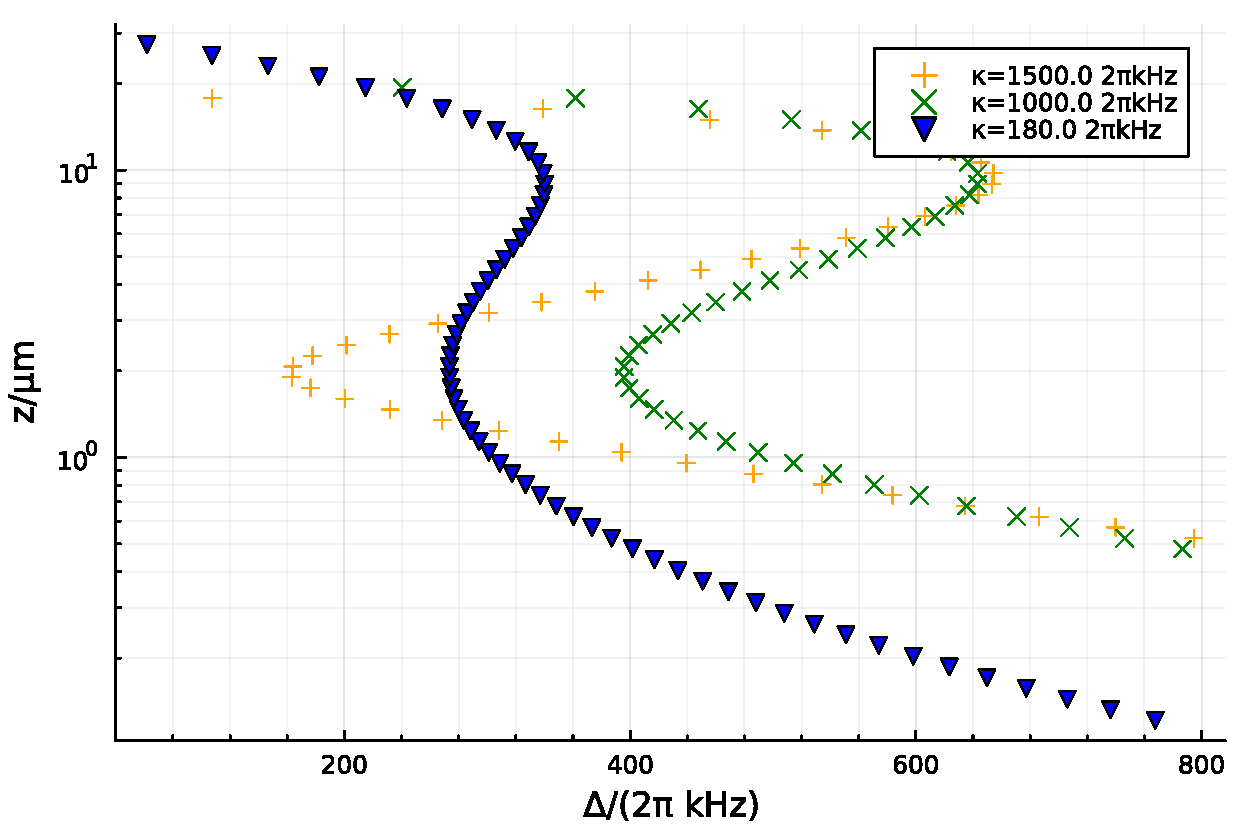
\includegraphics[width=.8\textwidth]{chapters/10_single_cavity/kappas.pdf}
    \caption{
        Plot of the equilibrium positions as a function of $z$ and $\Delta$ for multiple values of $\kappa$, with the parameters of Table \ref{tab:sp:sim:params}
    }
    \label{fig:sp:kappas}
\end{figure}
\begin{table}[!ht]
    \centering
    \begin{tabular}{|c|cl|}
        \hline
        \textbf{\shortstack{Laser \\Parameter}} & \textbf{Value}  & \\ \hline \hline
        $\lambda_0$&  $1150$ & $\unit{nm}$ \\ \hline
        $P_t$ & $0.5$ & $\unit{W}$ \\ \hline
        $W_t$  & $1$ & $\unit{\mu m}$ \\ \hline
        $A_x=A_y$ & $1$ &    \\ \hline
    \end{tabular}

    \begin{tabular}{|c|cl|}
        \hline
        \textbf{\shortstack{Particle \\Parameter}} & \textbf{Value} & \\
        \hline\hline 
        $\rho$ & $2200$ & $\unit{kg~m^{-3}}$ \\ \hline
        $\epsilon$ & $2.07$& \\ \hline
        $R$ & $100$ & $\unit{nm}$ \\ \hline
    \end{tabular}
    \begin{tabular}{|c|cl|}
        \hline
        \textbf{\shortstack{Cavity \\Parameter}} & \textbf{Value} & \\
        \hline\hline 
        $W_c$ & $20$ & $\unit{\mu m}$ \\ \hline
        $L_c$ & $19.8$ & $\unit{mm}$ \\ \hline
        $\zeta$ & $1$ & \\ \hline
    \end{tabular}
    
    \caption{
        Parameters of the calculation for one particle.\\
        The parameters are taken from Reference \cite{Gonzalez_Ballestero_2019}
        }
    \label{tab:sp:sim:params}
\end{table}
From the plots, it can be observed that the curve for the detuning $\Delta(z)$ with fixed $\kappa$ follows the characteristic inverse ``S'' shape that can be observed in cubic polynomials.
Also, notably this gives us configurations with multiple equilibrium positions.
In the plot, it can be seen that,
    with an increasing $\kappa$, 
    the curve gets flatter and the vertices get further apart as compared to less $\kappa$.
This implies a decreased sensitivity to detuning, 
    which manifests as a wider spacing between the vertices.

Extrapolating this for $\kappa \rightarrow \infty$, the curve would collapse into a single line at $z = 0$.
This behavior is consistent with our analytical prediction in Section \ref{sec:sp:specialcases}.
Conversely, for $\kappa \rightarrow 0$ we would get that for every value of $\Delta$ there would only be a single value for $z$.
If we take this even further, the curve would tend to infinity at $\Delta = 0$ 
    and go to $z = 0$.
This also matches our prediction of this case in Section \ref{sec:sp:specialcases}.

We can also observe that the solutions tend to $0$ for larger detunings,
    which also matches the prediction of Section \ref{sec:sp:specialcases}.

The limiting behaviors confirm the validity of our calculation.
These results have never been predicted in literature.
Since one typically either assumes larger values for $\kappa$
    or has only access to larger values of $\kappa$ in experiments.


\section{Stability}
\label{sec:sp:stability}

For any experimental use case of this system, it would be important to know the stability of the equilibrium positions.
In this section, we will derive the stability of the generated equilibrium conditions.

We define $\vec\eta := [x, p_x, y, p_y, z, p_z, \alpha_c, \alpha_c^*]$,
    with this Hamilton's equation are
    \begin{equation}
    \dot{\vec\eta} = \mat{J} \cdot \grad_{\vec \eta} H - \mat{K}\cdot \vec\eta.
    \end{equation}
with $\mat{K}$ modeling the damping 
\begin{equation}
    \mat{K} = \Diag\left(0,\dots,0, -\frac\kappa2, -\frac\kappa2 \right).
\end{equation}
%Note that even though $\alpha_c^*$ is just the complex conjugate of $\alpha_c$,
%    formally we need to treat them as independent for the stability analysis.
To analyze the stability we can linearize the equation of motion around the equilibrium position $\vec\eta_0$
\begin{align}
    \dot{\vec\eta} 
    &= \mat{J} \cdot \grad_{\vec \eta} H - \mat{K}\cdot \vec\eta\\
    &= \mat{J} \cdot \left(  
        \grad_{\vec \eta}\grad_{\vec \eta}H(\vec\eta_0)  \cdot \vec\eta
    \right) + \O(\norm{\vec \eta}^2) - \mat{K}\cdot \vec\eta \\
    & \approx \mat{J} \cdot \Hess_{\vec \eta} H \cdot \vec\eta- \mat{K}\cdot \vec\eta \\
    & := \mat{S} \cdot\vec\eta,
\end{align}
Note that this $\mat{J}$ is not the canonical symplectic form usually found in classical mechanics,
    which is a result of our non-canonical transform in Section \ref{ssec:sp:Hc}.

To analyze the stability,
    we need to check the Eigenvalues of the Matrix $\mat{S}$.
The results will be superpositions of $\vec v_i \cdot\exp(\lambda_i\cdot t)$
    and for the system to be stable none of those may diverge to infinity, 
    i.e. the Eigenvalues need to satisfy $\Re\lambda_i \leq 0$.

Every first-order partial derivative of $H$ with $x$ or $y$  can be expressed as $\partial_i H = r_i h_i(\vec r),~i\in \{x,y\}$.
Since every equilibrium has $x = 0 = y$,
    we can argue that every partial derivative of $\partial_j \partial_i H = r_i \partial_j h_i(\vec r) = 0,~ i\in \{x,y\}, ~j \in \{x,y,z, \alpha_c, \alpha_c^*\},~j\neq i$ at $x=0=y$.
Furthermore, since the momentum only appears in the kinetic term,
    the every momentum derivative is $\partial_{p_i} H = p_i/m$.
In this ordering, the Hessian of the Hamiltonian can be written using a diagonal block matrix
\begin{equation}
    \Hess H = \begin{pmatrix}
        \mat{X} \\
        & \mat{Y} \\
        & & \mat{C}
    \end{pmatrix}.
\end{equation}
The matrices $\mat{X} \in \R^{2\times 2}$ and $\mat{Y} \in \R^{2\times 2}$ are the Hessians of the $x, p_x$ and $y, p_y$ subspaces respectively, 
    the matrix $\mat{C} \in \C^{4\times 4}$ is the Hessian with respect to the remaining coordinates.

Our symplectic structure is
\begin{equation}
    \mat{J} = \begin{pmatrix}
        \mat{j} \\
        & \mat{j}\\
        & & \mat{j} \\
        & & & \tfrac1{\i \hbar}\mat{j}
    \end{pmatrix},~\mat{j} = \begin{pmatrix}
        0 & 1\\ -1 & 0 
    \end{pmatrix}.
\end{equation}

This gives the expression
\begin{equation}
    \mat{J}\cdot \Hess H = \begin{pmatrix}
        0 & \tfrac1m \\
        -\partial_x^2 H & 0\\
        & & 0 &\tfrac1m \\
        & &  -\partial_y^2 H & 0 \\
        & & & & \mat{B}
    \end{pmatrix},
\end{equation}
with
\begin{equation}
    \mat{B} = \begin{pmatrix}
        0 & \tfrac1m & 0 & 0 \\
        -\partial_z^2 H & 0 & -\partial_z\partial_{\alpha_c} H 
            & -\partial_z\partial_{\alpha_c^*} H \\
        \tfrac{1}{\i\hbar} \partial_z\partial_{\alpha_c^*} H 
            & 0 & \tfrac{1}{\i\hbar} \partial_{\alpha_c}\partial_{\alpha_c^*} H & 0\\
        -\tfrac{1}{\i\hbar}\partial_z \partial_{\alpha_c} H
            & 0 & 0 & -\tfrac{1}{\i\hbar} H \partial_{\alpha_c}\partial_{\alpha_c^*} H
    \end{pmatrix}.
\end{equation}
By Laplace expansion of the by $\lambda$ shifted matrix,
    it is observed that the $x$ and $y$ components decouple completely.
This means that we can get the eigenvalues of each block of the matrix individually.
Formally this is stated as
\begin{equation}
    \left| \mat{j}\cdot \mat{X}- \Id \lambda \right| \cdot \left| \mat{j}\cdot \mat{Y}- \Id \lambda \right| \cdot \left| \mat{B} - \Id \lambda \right| \overset{!}{=} 0.
\end{equation}

We get that Eigenvalues of the decoupled $x$ and $y$ components are
\begin{equation}
    \lambda = \pm \i\sqrt{\frac{\partial_i^2H}m}~, i \in \{x,y\}.
\end{equation}
It is trivial to see that the stability criterion for those components is 
    $\partial_i^2H > 0$.
From our computation of the gradients in Sections \ref{ssec:sp:extrem:x} and \ref{ssec:sp:extrem:y}
    the derivatives take the form $\partial_i H = r_i h_i(\vec r)$,
    where we call $r_x = x$ and $r_y = y$.
The second derivative can be computed to $\partial_i^2H = h_i(\vec r)$,
    which is given by the analytic computations.
We check the stability of $\mat{X}$ and $\mat{Y}$ from the analytic results,
    and we compute the Hessian with respect to $[z, p_z, \alpha_c, \alpha_c^*]$ numerically.
Since we cannot compute the numeric derivatives of a complex variable numerically,
    we need to transform the Hessian of our matrix,
    the formalism for this is described in the Appendix in Section \ref{apdx:sp:hessian:1d}.
With this transform, we can take the numeric derivative of our Hamiltonian. 
We do this using the \pkg[1.3]{ForwardDiff.jl} \cite{FWDiff-Cite} package.
The result of the stability check can be seen in Figure \ref{fig:sp:stability}.

We can observe that the system is always stable,
    in the considered parameter regime.

An interesting special case for the stability analysis
    is if $\alpha_c$ reaches its equilibrium position instantaneously.
The Analysis for this system is done in the Appendix under Section \ref{apdx:sp:fcf}.
However, the Cavity needs several round-trips between the mirrors to reach its equilibrium state
    and thus, this approximation does not hold in our system.

\begin{figure}%[h]
    \centering
    %\input{chapters/10_single_cavity/stabilities}
    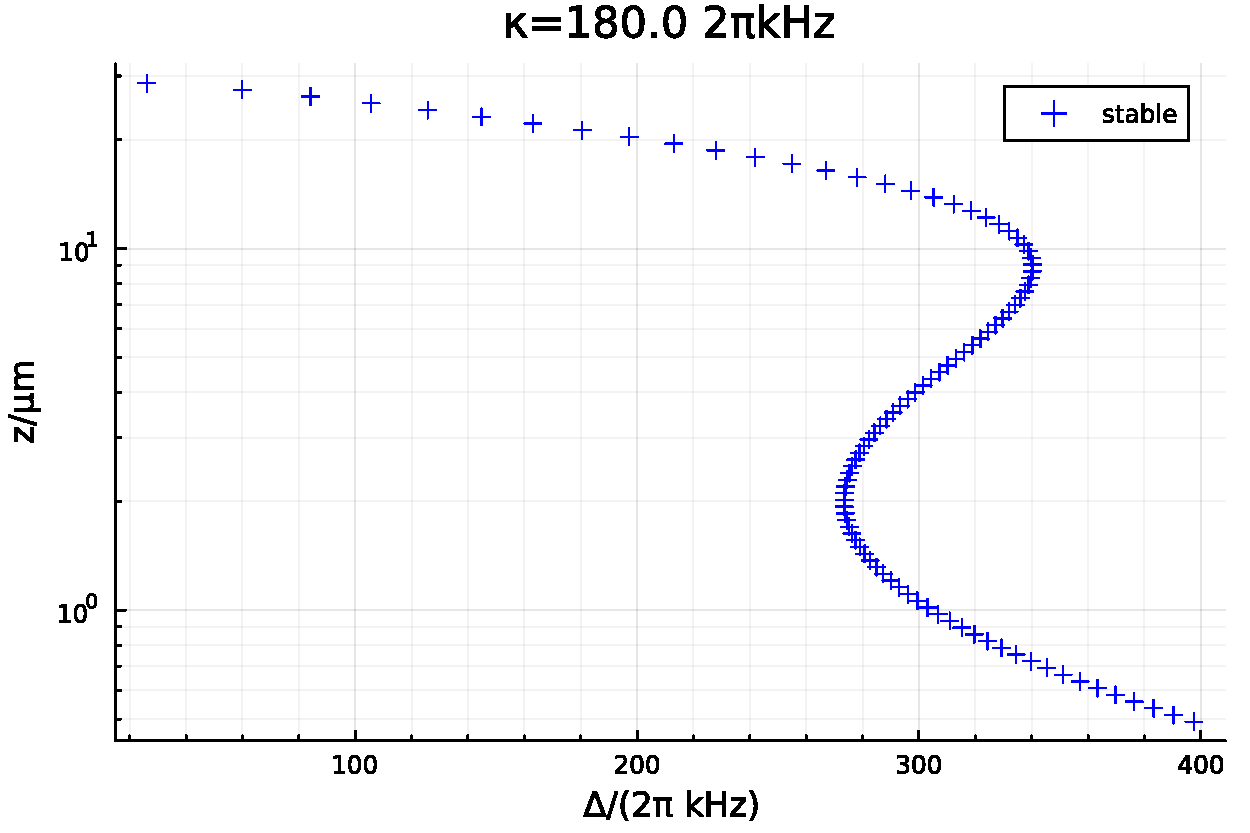
\includegraphics[width=.8\textwidth]{chapters/10_single_cavity/stabilities.pdf}
    \caption{
    Plot of the equilibrium position at $\kappa = 180.0 ~ 2\pi kHz$\\ 
    showing the stability of the equilibrium points\\ 
    with the parameters of Table \ref{tab:sp:sim:params}
    }
    \label{fig:sp:stability}
\end{figure}